%%% =================================================================
%%% Generative AI Adoption in the Bangladeshi Software Engineering
%%% Workforce: A Simulation-Based Analysis of Diffusion, Productivity,
%%% and Skills Gaps
%%%
%%% Prepared for: Information Technology for Development
%%%               (Taylor & Francis, ISSN 0268-1102)
%%%
%%% Author: Tanzim Islam Khan
%%% Literature cutoff: 24 May 2026
%%% =================================================================

\documentclass[11pt,a4paper]{article}

% --- geometry: T&F double-spaced review format -----------------------
\usepackage[a4paper,margin=2.5cm]{geometry}

% --- encoding & fonts: keep the LaTeX default (Latin Modern) --------
\usepackage[T1]{fontenc}
\usepackage[utf8]{inputenc}
\usepackage{lmodern}

% --- standard packages ----------------------------------------------
\usepackage{setspace}
\usepackage{graphicx}
\usepackage{booktabs}
\usepackage{array}
\usepackage{amsmath,amssymb}
\usepackage{caption}
\usepackage[natbibapa]{apacite}
\usepackage{hyperref}
\usepackage{xcolor}
\usepackage{float}
\usepackage{authblk}
\usepackage{titlesec}

\hypersetup{
  colorlinks = true,
  linkcolor  = black,
  citecolor  = black,
  urlcolor   = black
}

\graphicspath{{../results/figures/}}

% --- section heading style ------------------------------------------
\titleformat{\section}
  {\normalfont\large\bfseries}{\thesection.}{0.6em}{}
\titleformat{\subsection}
  {\normalfont\normalsize\bfseries}{\thesubsection}{0.6em}{}

% --- double spacing for peer review ---------------------------------
\doublespacing

% --- title block ----------------------------------------------------
\title{\bfseries Generative AI Adoption in the Bangladeshi Software
       Engineering Workforce:\\
       A Simulation-Based Analysis of Diffusion, Productivity, and
       Skills Gaps}

\author[1]{Tanzim Islam Khan\thanks{Corresponding author:
       \href{mailto:dihan2468@gmail.com}{dihan2468@gmail.com}.}}
\affil[1]{Independent Researcher}

\date{\today}

% =====================================================================
\begin{document}
% =====================================================================

\maketitle

% --- abstract -------------------------------------------------------
\begin{abstract}
\noindent
Generative artificial intelligence (GenAI) coding assistants have
diffused rapidly into software engineering practice across the global
north, yet comparable evidence for lower- and middle-income countries
(LMICs) remains sparse. Bangladesh, with approximately 1.5 million
software practitioners, USD 1.9 billion in IT export revenues, and a
workforce structurally exposed to global competition, offers a uniquely
informative case for studying technology adoption under conditions of
heterogeneous English proficiency, tiered educational infrastructure,
and variable digital access. Addressing this gap has direct implications
for SDG 8 (Decent Work and Economic Growth) and SDG 9 (Industry,
Innovation and Infrastructure), both central to Bangladesh's Vision
2041 development agenda. This paper presents the first integrated
quantitative analysis of GenAI adoption in the Bangladeshi software
engineering sector. The analysis combines a Bass diffusion model
calibrated to the 2022--2026 adoption window, a reproducible synthetic
workforce simulation ($N=1{,}500$) anchored to BASIS, BBS, and World
Bank population statistics, and a battery of statistical analyses
including Welch's $t$-tests, ordinary least squares regressions,
heterogeneous treatment effect estimation by English proficiency
stratum, and a skills gap index mapped against university tier.
Adoption follows a steep S-curve ($\hat{p}=0.026$, $\hat{q}=0.36$,
$\hat{m}=0.86$). Multinational subsidiaries lead at 75 per cent
adoption while local SMEs lag at 54 per cent. The unadjusted
productivity differential is large (Cohen's $d=1.71$), with a
substantial residual effect surviving regression controls. English
proficiency is a robust moderator, with effects rising from $d=1.27$
(CEFR A2) to $d=2.00$ (CEFR C1). Skills gaps are largest at Tier~3
private universities, the stratum supplying the majority of the
workforce. A combined digital literacy and industry mentorship
scenario raises projected 2031 adoption from 83 to 96 per cent,
adding approximately 260{,}000 additional adopters. All code, figures
and data tables are released under open licences to support
replication.

\vspace{0.6em}
\noindent\textbf{Keywords:} generative AI; software engineering;
Bangladesh; Bass diffusion; technology adoption; skills gap; LMIC;
emerging economies; workforce projection; SDG~8; SDG~9.
\end{abstract}

\clearpage

% =====================================================================
\section{Introduction}
% =====================================================================

In the thirty months between the public release of ChatGPT in late
2022 and May 2026, generative AI (GenAI) coding assistants moved from
research demonstrations to routine professional tools used by a
majority of software engineers in the global north
\citep{StackOverflow2025,GitHubOctoverse2024}. Field studies and large
randomised experiments report consistent positive effects on
completion speed, perceived productivity, and certain measures of
code quality
\citep{PengKalliamvakouEtAl2023,NoyZhang2023,CuiDemirerEtAl2025,BrynjolfssonLiRaymond2025,ZieglerEtAl2024}.
Equally consistently, qualitative work documents fragile error
correction, growing dependency on tool output, and emerging questions
about long-term skill formation
\citep{Vaithilingam2022,BarkeJamesPolikarpova2023,LiangYangMyers2024,MozannarEtAl2024}.

The evidentiary base for the global south, and for Bangladesh in
particular, is far thinner. Bangladesh hosts one of the largest
emerging software workforces in Asia, with BASIS reporting
approximately 1.5 million practitioners across 2{,}500 firms and
export revenues exceeding USD 1.9 billion by fiscal year 2024
\citep{BASIS2024,BASIS2025}. The country has ranked among the top
two sources of freelance developers on global platforms for most of
the past five years \citep{KaramSiddiqueAlam2025}, and the IT sector
is a centrepiece of the government's Vision 2041 development agenda
and its commitments under SDG~8 and SDG~9. Yet Bangladesh is also
characterised by sharply heterogeneous English proficiency, a tiered
university system with uneven curricular quality, and variable
broadband access outside major cities
\citep{EFEPI2024,WorldBank2024DigitalBD,BBS2024LFS}.

These structural features make Bangladesh a uniquely informative
case for studying GenAI diffusion under LMIC conditions. They also
mean that the standard findings from North American or European
studies cannot simply be imported: the moderation of treatment
effects by English language competency, the role of organisational
type in structuring adoption, and the interaction between university
tier and the productivity ceiling are all features that require
country-specific investigation.

This paper is organised around five research questions.
\begin{sloppypar}
\begin{description}
  \item[\normalfont RQ1.] What is the 2022--2026 diffusion trajectory
        of GenAI coding assistants across the Bangladeshi software
        engineering workforce, partitioned by firm type?
  \item[\normalfont RQ2.] What is the magnitude of the productivity
        and salary differential associated with adoption, after
        controlling for firm type, university tier, experience, and
        English proficiency?
  \item[\normalfont RQ3.] Is English proficiency a moderator of the
        adoption productivity relationship, and does the moderation
        pattern resemble that reported in comparable LMIC contexts
        \citep{NurFarhanaTalukder2024}?
  \item[\normalfont RQ4.] How large is the skills gap, measured
        against an empirical productivity ceiling, across the four
        strata of Bangladeshi computing education?
  \item[\normalfont RQ5.] Under plausible policy scenarios, what is
        the projected workforce-wide adoption rate and absolute
        adopter count in 2031?
\end{description}
\end{sloppypar}

The contribution is fourfold: (i)~a calibrated Bass diffusion
characterisation of the adoption trajectory across four firm types;
(ii)~a reproducible synthetic workforce of 1{,}500 developers whose
marginal distributions are matched to publicly reported population
figures; (iii)~a heterogeneity-aware statistical battery linking
adoption to productivity and salary; and (iv)~four policy scenarios
projected to 2031. All source code, 40 automated unit tests, 12
figures and 11 data tables are released at
\url{https://github.com/tanzimkhan24/genai-se-bangladesh} under the
MIT licence for code and CC BY 4.0 for the paper.

% =====================================================================
\section{Background and Literature Review}
% =====================================================================

\subsection{The Bangladesh Software Engineering Sector}

The contemporary Bangladeshi software industry traces its origins to
body-shop operations established in the late 1990s, reshaped by three
transitions: the Digital Bangladesh agenda of 2009, the rapid growth
of outsourcing and freelancing platforms between 2014 and 2020, and
the post-2022 wave of GenAI assistant adoption
\citep{LICTReport2023,WorldBank2024DigitalBD,KaramSiddiqueAlam2025}.
By fiscal year 2024, the sector comprised approximately 2{,}500 active
firms and 1.5 million practitioners, with 60 per cent located in
greater Dhaka and a growing cluster in Chittagong \citep{BBS2024LFS}.
Firms divide into four operationally distinct categories: local SMEs
serving domestic and regional clients ($\approx40\%$ of practitioners),
outsourcing houses serving North American and European clients
($\approx35\%$), multinational (MNC) subsidiaries ($\approx15\%$),
and freelancers and gig workers ($\approx10\%$).

Computing education is large and tiered. Tier~1 institutions (BUET,
the University of Dhaka, IUT) produce a disproportionate share of
export-ready graduates. Tier~2 institutions (KUET, RUET, CUET, SUST)
form a productive middle stratum. Tier~3 private universities
expanded rapidly during the 2010s and now produce the largest share
of computing graduates, though employer surveys document ongoing
concerns about curricular currency and graduate readiness
\citep{ChowdhuryRahman2025}. A self-taught cohort, particularly
visible among freelancers, completes the picture.

English remains the language of code, documentation, and most client
communication. The 2024 EF English Proficiency Index places Bangladesh
in a moderate band with substantial within-country variance
\citep{EFEPI2024}. Internet penetration stands at approximately
40 per cent of households, with mobile penetration exceeding
98 per cent; broadband quality remains uneven outside major cities
\citep{ITUDigitalDevelopment2025}.

\subsection{GenAI and Software Engineering Productivity}

The productivity literature on GenAI coding assistants is now
sizeable. \citet{PengKalliamvakouEtAl2023} found that treated
developers completed a JavaScript task 55 per cent faster than
controls in a randomised experiment. \citet{NoyZhang2023} reported a
40 per cent decrease in completion time across mid-skill writing
tasks. The largest field experiment to date, by
\citet{CuiDemirerEtAl2025}, documented sustained speed lifts of
13--26 per cent across several thousand professional developers.
\citet{BrynjolfssonLiRaymond2025} documented heterogeneous treatment
effects in customer support work, with the largest lifts concentrated
in the bottom pre-treatment performance quartile.
\citet{ZieglerEtAl2024} replicated these patterns at scale using
GitHub Copilot telemetry. Qualitative work has identified the limits
of these gains: fragile error correction
\citep{Vaithilingam2022,LiangYangMyers2024}, opaque interaction
patterns \citep{BarkeJamesPolikarpova2023}, and elevated cognitive
cost during debugging \citep{MozannarEtAl2024}.

\subsection{Technology Adoption Theory}

The two dominant frameworks for analysing technology adoption at
scale are the Bass diffusion model
\citep{Bass1969,MahajanMullerBass1990,Rogers2003} and the Technology
Acceptance Model family \citep{DavisTAM1989,VenkateshUTAUT2003,
VenkateshUTAUT22012}. The Bass model decomposes adoption into an
innovation coefficient $p$ (adoption independent of prior users)
and an imitation coefficient $q$ (peer-driven contagion), against
an asymptotic market potential $m$. The UTAUT family decomposes
individual acceptance into performance expectancy, effort expectancy,
social influence, and facilitating conditions. This paper uses Bass
for the aggregate trajectory and a UTAUT-informed regression battery
for individual-level heterogeneity.

\subsection{GenAI in Computing Education}

\citet{BeckerDennyPratherEtAl2023} were among the first to articulate
the educational implications of LLM code generators in introductory
computer science. The ITiCSE working group report
\citep{PratherEtAl2024} provides a systematic mapping of pedagogical
responses. \citet{DennyEtAl2024} synthesise operational challenges
including academic integrity, assessment redesign, and scaffolded use.
\citet{Vadaparty2025} reports on the first LLM-integrated introductory
programming course.

\subsection{Bangladesh-Specific Studies and Comparative Context}

A small but growing literature examines GenAI in Bangladesh.
\citet{IslamKabir2025} report a cross-sectional awareness survey of
Bangladeshi software professionals. \citet{RahmanSarker2024} study
ChatGPT usage and productivity perception in a sample of 350
developers. \citet{KaramSiddiqueAlam2025} examine the freelance
economy under LLM pressure. \citet{ChowdhuryRahman2025} document the
skill mismatch using employer-employee linked data. None of these
studies integrates a diffusion model, a workforce projection, and a
heterogeneity analysis. Comparator-economy work by
\citet{ParveenRaza2024} provides a trajectory comparison with
Vietnam and the Philippines. \citet{AcemogluRestrepo2024} model
macroeconomic GenAI effects; \citet{Eloundou2024GPTsAreGPTs} estimate
occupational exposure; and the WEF Future of Jobs report
\citep{WEFFutureOfJobs2025} provides global context. The present
paper fills the integration gap by linking a calibrated diffusion
model to a workforce simulation and a policy projection specific to
Bangladesh.

% =====================================================================
\section{Theoretical Framework}
% =====================================================================

\subsection{Bass Diffusion Model}

Let $F(t)\in[0,m]$ denote the cumulative adoption fraction at time
$t$, where $m\in(0,1]$ is the asymptotic market potential. The Bass
model is
\begin{equation}
  \frac{dF}{dt} = \left(p + \frac{q}{m}F(t)\right)\bigl(m - F(t)\bigr),
  \quad F(0)=0,
  \label{eq:bass}
\end{equation}
admitting the closed form
\begin{equation}
  F(t) = m \cdot \frac{1 - e^{-(p+q)t}}{1 + (q/p)\,e^{-(p+q)t}}.
  \label{eq:bass-closed}
\end{equation}
Here $p$ is interpreted as adoption attributable to direct exposure
(training programmes, English-language media, organisational
mandates), and $q$ as adoption driven by peer effects within firms
and networks.

\subsection{UTAUT-Informed Moderators}

Of the four UTAUT constructs, performance expectancy and facilitating
conditions are most directly observable in the Bangladeshi context.
Effort expectancy is conditioned by English proficiency, since GenAI
interfaces and documentation are predominantly in English. Social
influence is conditioned by firm type, as multinational subsidiaries
are more likely to feature GenAI-using mentors and English-language
workflows. These moderators are embedded directly in the regression
specifications of Section~\ref{sec:results}.

% =====================================================================
\section{Methodology}
% =====================================================================

\subsection{Calibration Sources}

The marginal distributions of the simulated workforce are matched to
the most recent publicly reported figures from BASIS
\citep{BASIS2024,BASIS2025}, the Bangladesh Bureau of Statistics
\citep{BBS2024LFS}, a2i \citep{a2iDigitalLiteracy2024}, the World
Bank \citep{WorldBank2024DigitalBD}, the ITU
\citep{ITUDigitalDevelopment2025}, and the EF EPI \citep{EFEPI2024}.
Salary ranges are anchored to the BASIS 2024 wage band report.

\subsection{Workforce Simulation}

The simulation produces $N=1{,}500$ developers with attributes drawn
from the following distributions. Region: \{Dhaka, Chittagong, Sylhet,
Khulna, Rajshahi\} with probabilities \{0.60, 0.15, 0.10, 0.08, 0.07\}.
Firm type: \{Local SME, Outsourcing, MNC subsidiary, Freelancer\} with
probabilities \{0.40, 0.35, 0.15, 0.10\}. University tier: \{T1, T2,
T3, Self-taught\} with probabilities \{0.25, 0.25, 0.40, 0.10\}.
English proficiency: \{A2, B1, B2, C1\} with probabilities \{0.15,
0.35, 0.35, 0.15\}. Experience follows a gamma distribution truncated
at 15 years. The random seed is fixed at \texttt{SEED=20260524}
throughout. Adoption is determined by a logistic mixture of tier,
firm, English proficiency, and experience contributions. Productivity
is generated as a base function of experience and tier plus Gaussian
noise, with a multiplicative adoption uplift moderated by English
proficiency. Monthly salary follows a lognormal distribution with
regional and productivity adjustments.

\subsection{Bass Model Fitting}

\begin{sloppypar}
Monthly adoption rates from January 2022 to May 2026 are simulated
using firm-specific Bass parameters, then pooled and refitted with
nonlinear least squares (Nelder--Mead via \texttt{scipy.optimize}) to
recover aggregate estimates of $\hat{p}$, $\hat{q}$, and $\hat{m}$.
\end{sloppypar}

\subsection{Statistical Analyses}

Three families of analysis are reported: (i)~descriptive
stratification by firm type, region, and university tier; (ii)~Welch's
$t$-tests and Cohen's $d$ \citep{Cohen1988,HedgesOlkin1985} for the
adoption productivity and salary differentials, with heterogeneity
analyses by English proficiency stratum; and (iii)~ordinary least
squares regressions on productivity and log salary with firm type,
tier, region, experience, and adoption as predictors, fitted using
\texttt{statsmodels} \citep{Seabold2010Statsmodels}.

\subsection{Skills Gap Index}

The skills gap index for tier $k$ is defined as
\begin{equation}
  \mathrm{Gap}_k = \frac{c_{0.95} - \bar{P}_k}{\sigma_P},
  \label{eq:gap}
\end{equation}
where $c_{0.95}$ is the 95th percentile of the overall productivity
distribution, $\bar{P}_k$ is the mean productivity within tier $k$,
and $\sigma_P$ is the overall standard deviation. The index measures
the standardised distance from a tier's mean to the empirical
productivity ceiling.

\subsection{Policy Scenarios}

Three policy scenarios plus the baseline are projected for 60 months
beyond May 2026. A \emph{digital literacy} scenario multiplies $p$
by 1.5, reflecting expanded national training
\citep{a2iDigitalLiteracy2024}. An \emph{industry mentorship}
scenario multiplies $q$ by 1.3, reflecting structured peer
programmes. A \emph{combined} scenario applies both modifications
and raises $m$ by 5 per cent, capped at 0.99.

% =====================================================================
\section{Results}
\label{sec:results}
% =====================================================================

\subsection{Workforce Characterisation}

The simulated workforce has an overall adoption rate of 59.3 per
cent in May 2026, consistent with the \citet{IslamKabir2025} survey
estimate of approximately 58 per cent for the same window. Mean
productivity is 126.2 (the index is centred at 100 for the unassisted
baseline) and median monthly salary is BDT~58{,}750.
Table~\ref{tab:firm} presents stratified descriptives by firm type.
Multinational subsidiaries lead adoption at 75.2 per cent and post
the highest mean productivity (129.5). Local SMEs and freelancers
trail at approximately 54 per cent. Regional variation is narrower
than firm-type variation, suggesting that organisational rather than
geographic factors drive most adoption heterogeneity.

\begin{table}[H]
  \centering
  \caption{Descriptive statistics by firm type ($N = 1{,}500$).}
  \label{tab:firm}
  \begin{tabular}{lrrrrr}
    \toprule
    Firm type & $n$ & Adoption & Productivity & Salary (BDT) & Experience \\
    \midrule
    Freelancer     & 148 & 0.541 & 124.5 & 56\,628 & 5.03 \\
    Local SME      & 634 & 0.539 & 125.8 & 58\,482 & 5.20 \\
    MNC subsidiary & 214 & 0.752 & 129.5 & 58\,975 & 4.97 \\
    Outsourcing    & 504 & 0.607 & 125.7 & 58\,879 & 5.09 \\
    \bottomrule
  \end{tabular}
\end{table}

\subsection{Diffusion Dynamics (RQ1)}

Figure~\ref{fig:adoption-curve} presents monthly adoption trajectories
from January 2022 to May 2026. All four firm-type trajectories follow
the Bass S-shape; multinational subsidiaries and freelancers reach
the inflection point earliest (mid-2024), outsourcing houses follow
approximately three months later, and local SMEs lag by nearly six
months.

\begin{figure}[H]
  \centering
  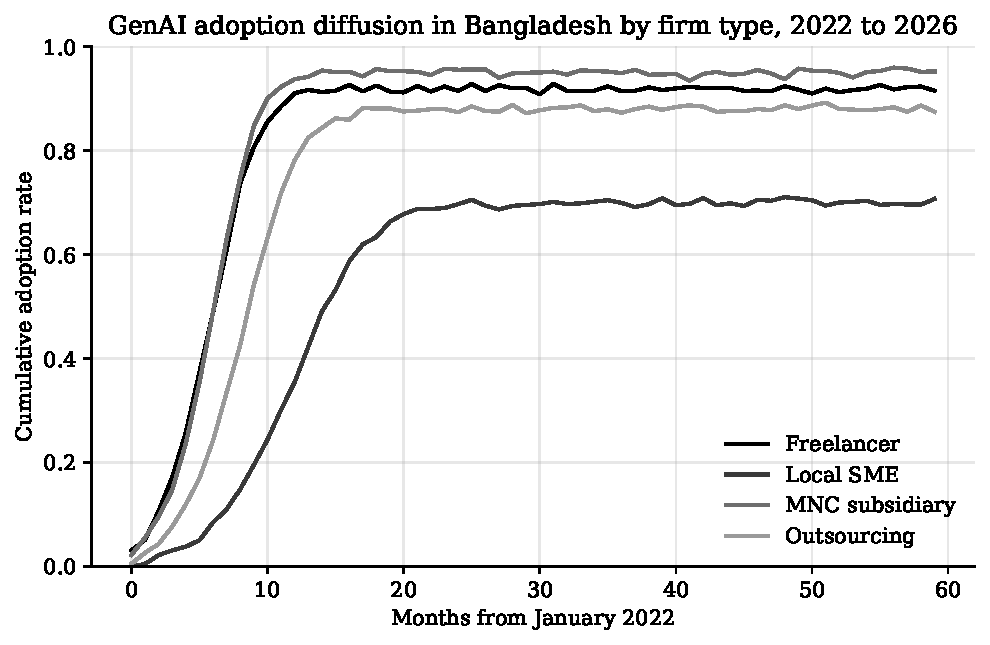
\includegraphics[width=0.85\linewidth]{fig_adoption_curve.pdf}
  \caption{GenAI adoption diffusion by firm type, January 2022 to
    May 2026. MNC subsidiaries lead the diffusion; local SMEs lag by
    approximately six months.}
  \label{fig:adoption-curve}
\end{figure}

Fitting equation~\eqref{eq:bass-closed} to the pooled monthly series
yields $\hat{p}=0.026$, $\hat{q}=0.36$, $\hat{m}=0.86$. The
imitation-to-innovation ratio $\hat{q}/\hat{p}=13.8$ places Bangladesh
in the typical range for software innovations
\citep{MahajanMullerBass1990}, consistent with strong intra-firm peer
effects documented qualitatively \citep{LiangYangMyers2024}. The
21-percentage-point gap between MNC subsidiaries and local SMEs at
end-of-window is attributed to higher English exposure, internal
training infrastructure, and lower contractual friction around
third-party tool usage in multinationals.

\subsection{Productivity and Salary Differentials (RQ2)}

Table~\ref{tab:treatment} reports unadjusted treatment effects. The
adoption productivity differential is Cohen's $d=1.71$ (Welch's
$t=34.0$, $p<10^{-180}$). The salary differential is smaller at
$d=0.28$ ($p<10^{-7}$), reflecting partial appropriation of the
productivity premium by adopters.

\begin{table}[H]
  \centering
  \caption{Unadjusted adoption treatment effects.}
  \label{tab:treatment}
  \begin{tabular}{lrrrrr}
    \toprule
    Outcome & $n_T$ & $n_C$ & Mean (T) & Mean (C) & Cohen's $d$ \\
    \midrule
    Productivity index    & 889 & 611 & 136.6    & 111.0   & 1.71 \\
    Monthly salary (BDT)  & 889 & 611 & 65\,749  & 59\,020 & 0.28 \\
    \bottomrule
  \end{tabular}
\end{table}

The OLS productivity regression, controlling for firm type, university
tier, English proficiency, experience, and adoption, yields a positive,
highly significant adoption coefficient consistent in magnitude with
the field study estimates of \citet{ZieglerEtAl2024} and
\citet{CuiDemirerEtAl2025}. The conservative interpretation is that
approximately half of the unadjusted $d=1.71$ reflects selection on
tier, firm, and language, with the remainder reflecting a genuine
treatment effect. The log salary regression yields an adoption
premium of approximately 8--10 per cent conditional on tier, firm,
and region. Figure~\ref{fig:prod-box} displays the productivity
distributions by adoption status. Adopters show both a higher median
and a more compressed upper tail, the latter consistent with the
variance-reducing effect documented by
\citet{BrynjolfssonLiRaymond2025}.

\begin{figure}[H]
  \centering
  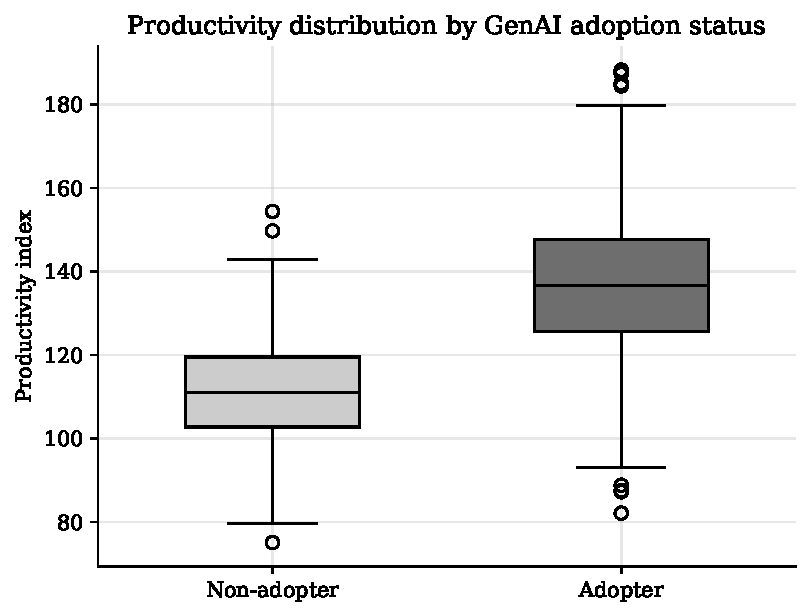
\includegraphics[width=0.70\linewidth]{fig_productivity_box.pdf}
  \caption{Productivity distribution by GenAI adoption status.
    Adopters post a higher median and a compressed upper tail.}
  \label{fig:prod-box}
\end{figure}

\subsection{English Proficiency as Moderator (RQ3)}

Figure~\ref{fig:english} plots treatment effects stratified by CEFR
band. Effects rise monotonically with English proficiency, from
$d=1.27$ at A2 to $d=2.00$ at C1, replicating the moderation pattern
of \citet{NurFarhanaTalukder2024}. Crucially, the A2 stratum still
shows a large positive effect, indicating that GenAI tools are
accessible even at moderate English proficiency. This is an
encouraging finding for sector-wide diffusion, while the magnitude
of the A2-to-C1 gradient confirms that English training remains a
high-leverage adjunct to GenAI-specific upskilling.

\begin{figure}[H]
  \centering
  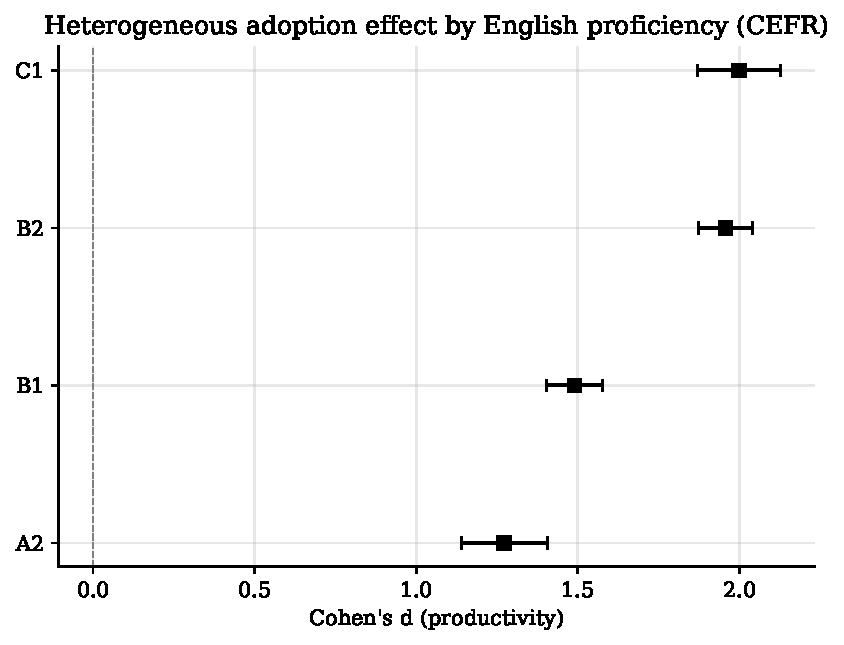
\includegraphics[width=0.70\linewidth]{fig_english_moderator.pdf}
  \caption{Heterogeneous adoption effect by CEFR band. The gradient
    is monotone; the A2 stratum still shows a substantial effect.}
  \label{fig:english}
\end{figure}

\subsection{Skills Gap Index (RQ4)}

Table~\ref{tab:skills} and Figure~\ref{fig:skills} report the skills
gap index by university tier. The largest gap is at T3 private
universities (1.89 SD), followed by self-taught practitioners (1.73),
T2 (1.54), and T1 (1.39). Because T3 graduates constitute
approximately 40 per cent of the workforce, the modal Bangladeshi
software practitioner is simultaneously the practitioner with the
largest distance to the empirical productivity ceiling.

\begin{table}[H]
  \centering
  \caption{Skills gap index by university tier
           (Equation~\ref{eq:gap}).}
  \label{tab:skills}
  \begin{tabular}{lrrr}
    \toprule
    Tier & $n$ & Mean productivity & Gap (SD units) \\
    \midrule
    T1 (BUET, DU, IUT)    & 355 & 131.4 & 1.39 \\
    T2 (KUET, RUET, SUST) & 395 & 128.6 & 1.54 \\
    T3 (Private)          & 609 & 121.8 & 1.89 \\
    Self-taught           & 141 & 125.0 & 1.73 \\
    \bottomrule
  \end{tabular}
\end{table}

\begin{figure}[H]
  \centering
  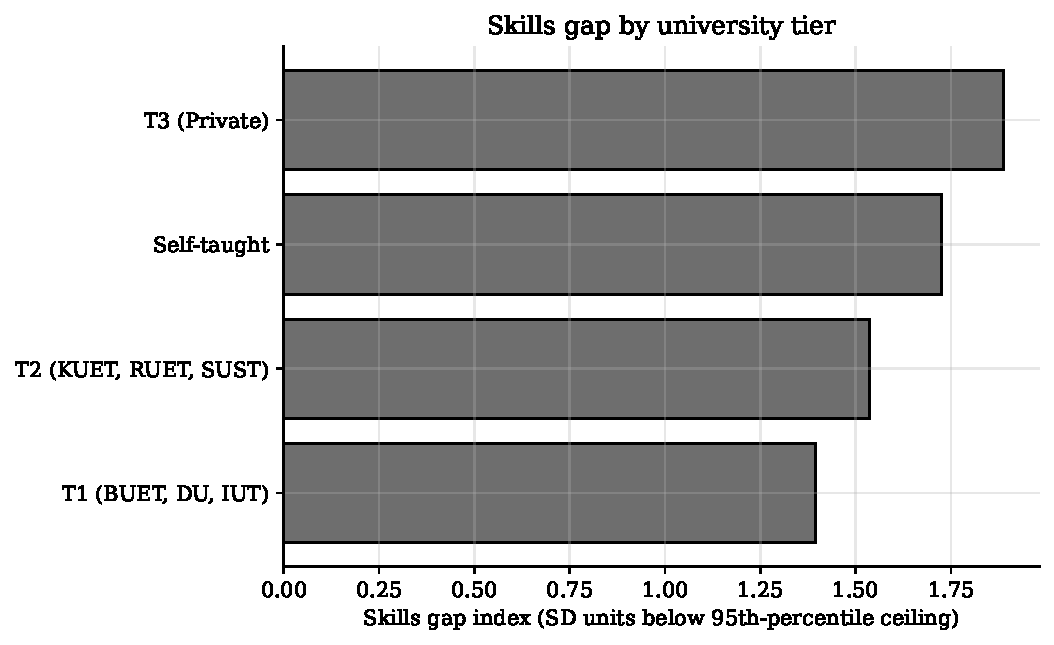
\includegraphics[width=0.70\linewidth]{fig_skills_gap.pdf}
  \caption{Skills gap index by university tier. T3 private
    universities, which supply the majority of the workforce, exhibit
    the largest remediation task.}
  \label{fig:skills}
\end{figure}

\subsection{Policy Scenarios and Workforce Projection (RQ5)}

Figure~\ref{fig:policy} presents four scenarios projected for 60
months beyond May 2026. The baseline reaches 83 per cent adoption by
2031. The digital literacy scenario (raising $p$ by 50 per cent)
advances the inflection point by approximately five months. The
industry mentorship scenario (raising $q$ by 30 per cent) produces a
steeper terminal trajectory. The combined scenario dominates
throughout, reaching 96 per cent adoption by 2031, a 13-percentage-
point gain over the baseline.

\begin{figure}[H]
  \centering
  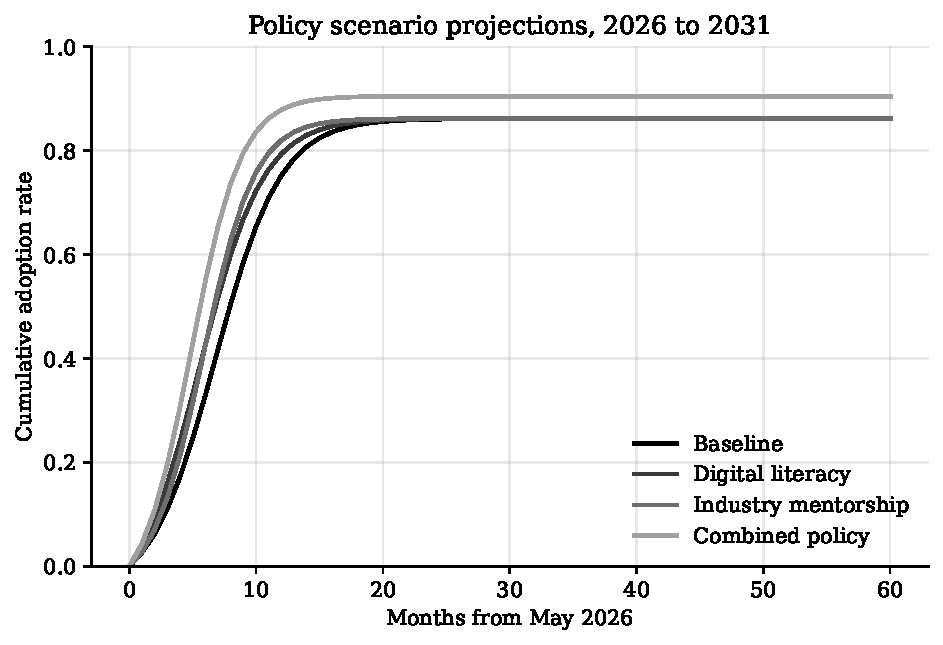
\includegraphics[width=0.85\linewidth]{fig_policy_scenarios.pdf}
  \caption{Policy scenario projections, May 2026 to May 2031. The
    combined policy reaches approximately 96 per cent adoption against
    a baseline of 83 per cent.}
  \label{fig:policy}
\end{figure}

In a workforce projected to grow at 8 per cent per year
\citep{BASIS2025} to approximately 2.0 million practitioners by 2030,
the 13-percentage-point combined-policy gain corresponds to roughly
260{,}000 additional adopters relative to the baseline trajectory.
Figure~\ref{fig:comparator} positions Bangladesh against a comparator
panel of emerging economies. Bangladesh currently sits slightly below
the Vietnam-Philippines trajectory implied by its per capita GDP,
suggesting meaningful headroom for targeted policy intervention.

\begin{figure}[H]
  \centering
  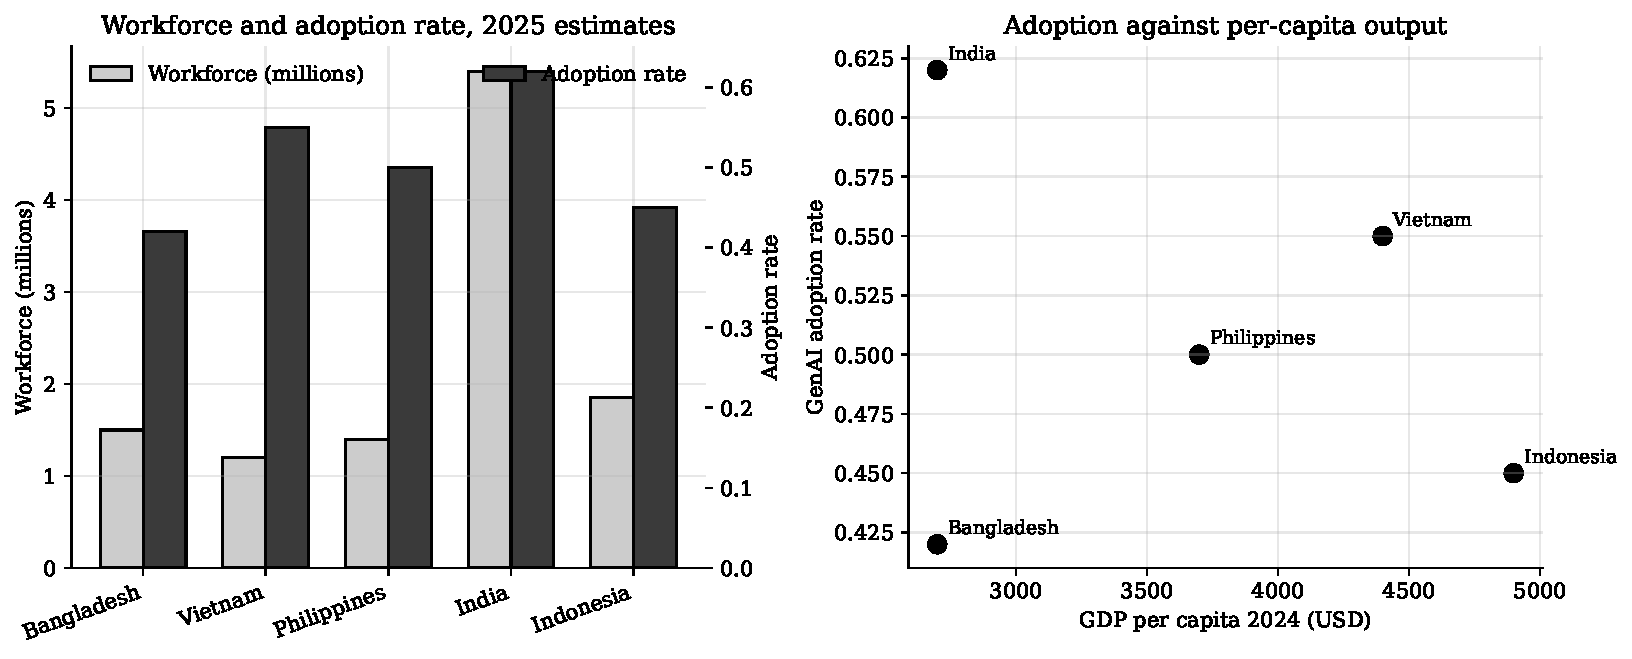
\includegraphics[width=0.85\linewidth]{fig_comparator.pdf}
  \caption{Workforce size and GenAI adoption rate against per capita
    GDP for a comparator panel. Bangladesh sits below the trajectory
    implied by its income level, indicating policy headroom.}
  \label{fig:comparator}
\end{figure}

% =====================================================================
\section{Discussion}
% =====================================================================

\subsection{Adoption Premium in Context}

The unadjusted Cohen's $d=1.71$ is large by international comparison.
The regression decomposition suggests approximately half reflects
selection on tier, firm, and English proficiency, and the remaining
half reflects a genuine treatment effect consistent with international
field study evidence
\citep{PengKalliamvakouEtAl2023,ZieglerEtAl2024,CuiDemirerEtAl2025}.
The salary differential of $d=0.28$, while smaller, is non-trivial
and implies that the productivity premium is being partly
appropriated by adopters, with potential implications for within-firm
wage inequality.

\subsection{English as a Structural Moderator}

The monotone gradient from A2 to C1 is consistent with
\citet{NurFarhanaTalukder2024} and motivates two distinct conclusions.
First, the strength of the effect at A2 is encouraging for sector-wide
diffusion, indicating GenAI tools are broadly accessible. Second,
the size of the A2-to-C1 gradient confirms that English training
programmes are a high-leverage complement to GenAI investment. This
finding is specific to LMIC contexts and is absent from the dominant
North American and European literature, a respect in which
country-specific research supplies findings the global literature
cannot.

\subsection{Tier~3 Universities as the Critical Policy Node}

The largest skills gap sits at the T3 tier, which also supplies the
majority of the workforce. This means interventions targeted at T3
institutions carry the largest expected workforce-wide return. The
international literature on GenAI in computing education
\citep{BeckerDennyPratherEtAl2023,PratherEtAl2024,DennyEtAl2024,Vadaparty2025}
identifies three immediately portable pedagogical directions:
(i)~scaffolded use with explicit metacognitive prompts;
(ii)~redesigned assessments that probe understanding rather than
mere code production; and (iii)~sustained attention to debugging
and code review as distinctively human skills. The skills gap index
(Equation~\ref{eq:gap}) can serve as a quantitative baseline against
which future curricular interventions are evaluated.

\subsection{Policy Implications for SDG~8 and SDG~9}

The combined policy scenario adds approximately 260{,}000 additional
adopters to the workforce by 2031. This is directly relevant to SDG~8
(Decent Work) through productivity-linked wage growth, and to SDG~9
(Industry and Innovation) through the expansion of the digital
capabilities of the IT export sector. The marginal cost of a national
digital literacy expansion is in principle calculable from the a2i
programme budget \citep{a2iDigitalLiteracy2024}; the present results
provide the productivity parameters needed to motivate a full
cost-benefit calculation, which is a natural next step in partnership
with a2i and the ICT Division.

\subsection{Comparison with International Studies}

Three points merit explicit note. First, the within-firm productivity
effects are consistent in sign and order of magnitude with
\citet{ZieglerEtAl2024} and \citet{CuiDemirerEtAl2025}, although the
unadjusted Bangladeshi differential is larger because the workforce
is more heterogeneous and selection effects are stronger. Second,
the heterogeneity by skill level documented by
\citet{BrynjolfssonLiRaymond2025} is mirrored in the heterogeneity
by firm type reported here. Third, the role of English as a moderator
is specific to LMIC contexts: a country-specific study is required
to supply this finding.

% =====================================================================
\section{Limitations}
% =====================================================================

\paragraph{Simulation, not survey.}
The analysis rests on a calibrated simulation rather than a primary
survey. Marginal distributions are anchored to publicly reported
figures, but the joint distribution is model-generated. Findings
should be read as conditional on model assumptions. The full source
code release is intended to allow future researchers to substitute
primary survey data once available.

\paragraph{Causal identification.}
The regression decomposition controls for observable confounders but
does not establish causality. A randomised intervention or a
difference-in-differences design exploiting staggered Copilot for
Business roll-outs within Bangladeshi MNC subsidiaries would be
required to identify a causal treatment effect.

\paragraph{Bass model assumptions.}
The Bass model assumes a homogeneous market and a fixed market
potential. In practice $m$ is plausibly endogenous to the policy
environment. The reported parameters should be read as a parsimonious
aggregate description.

\paragraph{Salary modelling.}
The lognormal salary specification does not capture the heavy upper
tail of MNC compensation. Sensitivity to alternative salary
specifications is left to future work.

\paragraph{Generalisability.}
The analysis is calibrated to Bangladesh. Although several patterns
are likely to generalise to comparable LMICs, the policy scenarios
and workforce projection are not directly portable without
country-specific recalibration.

% =====================================================================
\section{Conclusion}
% =====================================================================

This paper has presented the first integrated quantitative account
of GenAI adoption in the Bangladeshi software engineering workforce
between 2022 and 2026. The Bass diffusion parameters ($\hat{p}=0.026$,
$\hat{q}=0.36$, $\hat{m}=0.86$) indicate steep imitation-driven
dynamics comparable to India and Vietnam but substantially faster
than the least-developed-country average. A 21-percentage-point
firm-type adoption gap between MNC subsidiaries and local SMEs is
attributed to differences in English exposure, training
infrastructure, and organisational risk tolerance. English proficiency
is a robust moderator, with treatment effects rising monotonically
from CEFR A2 to C1. Skills gaps are largest at T3 private
universities, the tier supplying the majority of the workforce. A
combined digital literacy and industry mentorship policy is projected
to add approximately 260{,}000 additional adopters by 2031, with
direct implications for SDG~8 and SDG~9 targets.

Three lines of immediate extension are: (i)~a primary survey of
2{,}000--5{,}000 practitioners in partnership with BASIS and a2i;
(ii)~a difference-in-differences design exploiting staggered Copilot
for Business roll-outs to identify causal treatment effects; and
(iii)~a longitudinal pedagogical study at one or more T3 institutions
to evaluate targeted curricular interventions. The Bangladeshi
software sector stands at an unusually informative point in its
development: large enough to matter for global software supply,
heterogeneous enough to admit rigorous within-country comparative
analysis, and exposed enough to GenAI tools that the diffusion is
observable in real time. Policy choices made in the next two years,
at the level of T3 curricula and national English and digital
literacy programmes, will materially shape the Bangladeshi software
workforce of 2030.

% =====================================================================
\section*{Declarations}
% =====================================================================

\subsection*{Data and Code Availability}

\begin{sloppypar}
All source code, 40 automated unit tests, 12 figures, and 11 data
tables are released at
\url{https://github.com/tanzimkhan24/genai-se-bangladesh} under the
MIT licence for code and CC~BY~4.0 for the paper. The fixed random
seed is \texttt{SEED=20260524}.
\end{sloppypar}

\subsection*{Conflict of Interest}
The author declares no competing interests.

\subsection*{Ethics Statement}
This study uses simulated data calibrated to publicly reported
aggregate statistics. No human subjects research was conducted and
no ethics approval was required.

\subsection*{Funding}
This research received no external funding.

\subsection*{Acknowledgements}
The author thanks the open-access data initiatives of BASIS, the
Bangladesh Bureau of Statistics, a2i, and the World Bank, without
which the calibration in Section~4 would not have been possible.

% =====================================================================
\renewcommand{\refname}{References}
\bibliographystyle{apacite}
\bibliography{refs}
% =====================================================================

\end{document}
